\documentclass[11pt,letterpaper]{article}
\usepackage[margin=.9in]{geometry}
\usepackage[T1]{fontenc}
\usepackage{lmodern,microtype,amsmath,amssymb,amsthm,booktabs,tabularx,array}
\usepackage{tikz,fancyhdr,enumitem}
\usetikzlibrary{arrows.meta,positioning}
\usepackage[hidelinks]{hyperref}
\setlength{\parindent}{0pt}\setlength{\parskip}{5pt}\setlist{nosep,leftmargin=*}
\newtheorem{theorem}{Theorem}[section]
\newtheorem{proposition}[theorem]{Proposition}
\newtheorem{corollary}[theorem]{Corollary}
\theoremstyle{definition}\newtheorem{definition}[theorem]{Definition}\newtheorem{example}[theorem]{Example}\newtheorem{conjecture}[theorem]{Conjecture}
\newcommand{\E}{\mathbb E}\newcommand{\PP}{\mathbb P}\newcommand{\F}{\mathcal F}\newcommand{\Var}{\operatorname{Var}}\newcommand{\PC}{\operatorname{PC}}\newcommand{\N}{\mathbb N}
\pagestyle{fancy}\fancyhf{}\fancyhead[L]{\small The Professor of Professors}\fancyhead[R]{\small Atlas-audited draft 001v2}\fancyfoot[C]{\thepage}\setlength{\headheight}{14pt}
\title{\bfseries The Professor of Professors\\[4pt]\large Probabilistic Partial Credit, Recursive Awareness,\\and the Oracle Limit}
\author{Research Director: Brian Tenneson\\\small Mathematical development and drafting: Picard--CIIP\\\small (ChatGPT conversational research protocol)}
\date{26 November 2026 \quad | \quad Atlas-audited research draft 001v2}
\begin{document}
\maketitle
\begin{abstract}
The Professor of an automated theorem prover grades verified mathematical capital and geometric proximity to certified settlement. Its grade may be uncertain even though the verifier's acceptance rule is exact. We extend the transaction-geometric Professor to a hierarchy of probabilistic evaluators: a level-$n+1$ Professor assigns partial credit to level $n$ and revises the assessment of the original proof state. These tasks are deliberately distinct. For a frozen grading contract and nested admissible information, conditional expectations give a bounded martingale; squared-error ignorance decreases by the exact expected squared revision, and the limiting evaluator is the least-ignorance estimator relative to the accumulated information. Exact limiting grade recovery occurs almost surely precisely when the grade has a measurable version in that information. We also distinguish recursive evaluation from the acquisition of information, and exhibit a halting-encoded family whose computable finite-stage Professor grades have a limit function that is not uniformly computable in the instance index. An exact finite calculation compares informative and redundant Professors. The resulting architecture suggests an oracle limit without granting an evaluator authority over proof acceptance. The probabilistic results are conditional applications of established martingale theory; the proposed connection to oraclehood and settlement control is the research contribution under investigation.
\end{abstract}
\textbf{Central question.} If an ATP has a Professor, can that Professor itself be a student? If the answer is yes at every finite level, is the limiting Professor a Professor, an oracle, or neither?
\setcounter{tocdepth}{1}
\begingroup
\small
\makeatletter
\renewcommand*\l@section{\@dottedtocline{1}{0em}{1.5em}}
\makeatother
\tableofcontents
\endgroup
\clearpage
\section{From the original Professor to the recursive Professor}
The September 3 manuscript \emph{Partial Credit on Settlement Geometry} \cite{partial} defines a verifier-gated capital/geometry score. Sections 2--11 separate binary certificate acceptance, verified capital, the repair horizon, and the Professor's scalar projection. Section 12 distinguishes retrospective exact distances from unknown global distances. Most importantly, Section 24 proposes calibration awareness: an agent or controller should assess the reliability of the Professor's own feedback. The present draft promotes that observation to a recursive architecture. The parent paper is not amended in place.

Fix a role, a proof state $A$, a formal environment, a legal directed repair graph with nonnegative costs, a terminal set of accepted certificates, and a frozen relevance map $Q$. The original quantities are
\[
 q(A)=Q(A,K(A))\in[0,1],\quad H(A)=d(A,C)\in[0,\infty],\quad R(A)=e^{-H(A)/h},
\]
where $K(A)$ is the ledger of verified mathematical items, $h>0$, and $e^{-\infty}=0$. Write
\begin{equation}\label{eq:grade}
 Z=\alpha q+(1-\alpha)R,\qquad 0\leq\alpha\leq1.
\end{equation}
For each fixed fully specified instance this grade is a definite quantity; it need not be known or computable by the evaluator. The choice of $Q$, $\alpha$, $h$, the graph and the verifier must be stated. In particular, exactness relative to a grading contract is not a claim that the chosen scalarization is objectively optimal. The verified entries of $K$ and their possibly heuristic relevance weights remain separate. A score of one is not a certificate. Even $H=0$ need not imply membership in $C$ if zero-cost moves or unattained infima are allowed.

\begin{center}
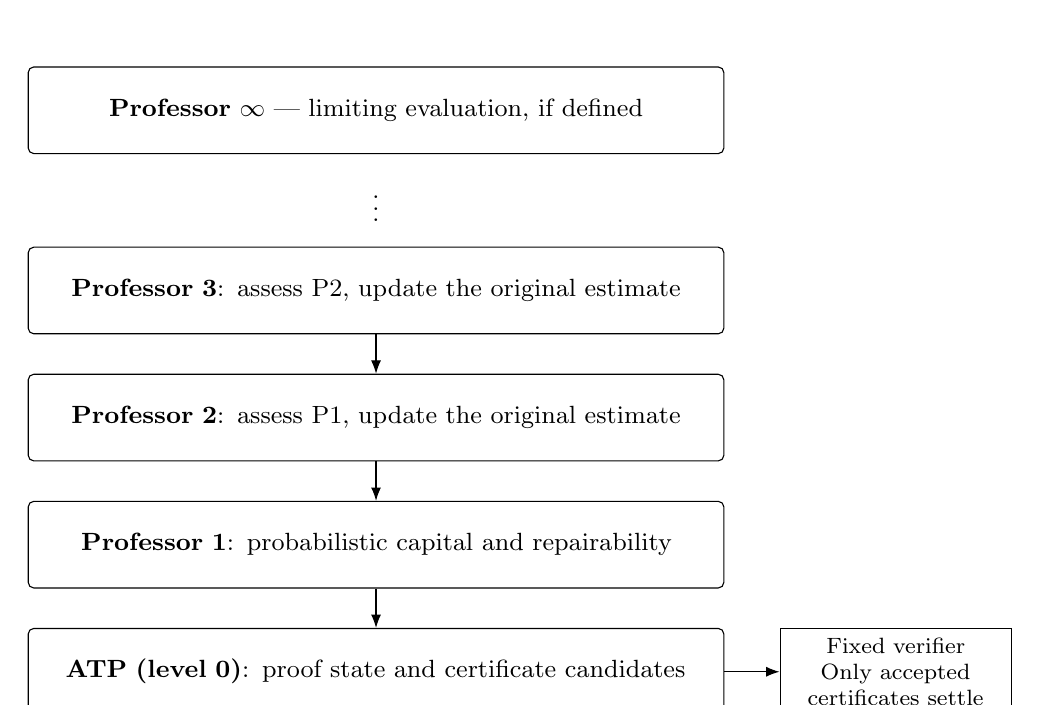
\begin{tikzpicture}[node distance=5mm,>=Latex, every node/.style={font=\small}, tier/.style={draw,rounded corners=2pt,text width=8.6cm,minimum height=11mm,align=center}]
\node[tier] (pinf) {\textbf{Professor $\infty$} --- limiting evaluation, if defined};
\node[below=2mm of pinf] (dots) {$\vdots$};
\node[tier,below=2mm of dots] (p3) {\textbf{Professor 3}: assess P2, update the original estimate};
\node[tier,below=of p3] (p2) {\textbf{Professor 2}: assess P1, update the original estimate};
\node[tier,below=of p2] (p1) {\textbf{Professor 1}: probabilistic capital and repairability};
\node[tier,below=of p1] (atp) {\textbf{ATP (level 0)}: proof state and certificate candidates};
\draw[->] (p3)--(p2);\draw[->] (p2)--(p1);\draw[->] (p1)--(atp);
\node[draw,align=center,font=\footnotesize,text width=2.7cm,right=7mm of atp] (v) {Fixed verifier\\Only accepted\\certificates settle};
\draw[->] (atp)--(v);
\end{tikzpicture}
\end{center}
\textit{Figure 1.} Assessment flows down the hierarchy. Authorized evidence may flow upward. Higher rank does not confer authority to change the verifier or admit a certificate.
\section{A probabilistic grading contract}
\subsection{One state, multiple possible worlds}
Let $(\Omega,\mathcal A,\PP)$ be a probability space of possible instances, hidden operational facts, and observations. The observed proof state and its admissible representation are fixed for the evaluation episode; uncertainty concerns which admissible instance is present or which facts about it are accessible. The measurable variables $q,R,Z$ take values in $[0,1]$. The identities are relative to a single declared probability law. To interpret their risks as actual population risks, that law must describe the target population; subjective confidence or agreement among graders does not establish this. Across possible instances the declared grading rule, $\alpha$ and $h$ are fixed constants, even if some facts determining $q$ and $H$ are hidden. A frozen public contract makes the meaning of $Z$ invariant across levels.

Let $\F_0\subseteq\F_1\subseteq\cdots\subseteq\mathcal A$ be a filtration of all information authorized for the aggregate evaluator through level $n$. It includes earlier reports, evidence, and any permitted randomness used in interpreting them. For a common-law ideal evaluator, conditional expectations are defined only up to null sets; choose measurable versions simultaneously for the countably many finite levels. The tower property concerns the aggregate information, not an assumption that every individual Professor sees all of it. New levels may inspect a certificate, compute a quotient bound, acquire a new independent observation, or reanalyze evidence. Reanalysis is valuable when it makes a previously inaccessible fact available; if it is just a measurable transformation of information already available in the idealized filtration, it adds no statistical information.
\begin{definition}[Probabilistic Professor]
The ideal level-$n$ report, for $n\geq1$, is the vector
\[
 (Q_n,R_n,P_n,V_n)=\big(\E[q\mid\F_n],\E[R\mid\F_n],\E[Z\mid\F_n],\Var(Z\mid\F_n)\big).
\]
Here $P_n=\alpha Q_n+(1-\alpha)R_n$. The capital coordinate is an estimate of the scalarized verified ledger, not a license to bank unverified items. If the ledger and its frozen scalarization are already known, that coordinate is observed exactly. The variance is uncertainty about the scalar grade, not a probability of certificate correctness. The finite implementation may return approximations, with separate evidence status and error bounds where available.
\end{definition}
A separate forecast may estimate $\PP(\tau\leq B\mid\F_n)$ for first certified settlement time $\tau$ under a frozen search policy and resource budget $B$. It is not the same as $P_n$. In particular, $\E[e^{-H/h}\mid\F_n]$ is not generally $e^{-\E[H\mid\F_n]/h}$ (and the latter may vanish if the mean horizon is infinite). The former preserves the original bounded coordinate.

\subsection{Partial credit on a Professor's answer}
Level $n+1$ receives the preceding report $P_n$, which is $\F_n$-measurable. Define its grade of that report by
\begin{equation}\label{eq:metagrade}
 G_{n+1}=1-\E[(Z-P_n)^2\mid\F_{n+1}].
\end{equation}
This is a conditional quadratic score for the preceding estimate, inspired by squared-error probability scoring \cite{brier}. It is meaningful for continuous grades as well as binary forecasts. Higher values reward smaller conditional expected squared errors. Since the grades lie in $[0,1]$, $G_{n+1}$ also lies in $[0,1]$. The expectation of the realized score $1-(Z-p)^2$ is uniquely maximized (up to null sets) by the conditional mean over measurable reports $p$; this does not score an entire predictive distribution or guarantee calibration of a practical grader. The new Professor also issues $P_{n+1}$, its own assessment of the original ATP state. For an actual preceding report $r_n\in[0,1]$ measurable in $\F_n$, the same definition with $r_n$ replacing $P_n$ grades that report; it need not be the ideal posterior mean.
\begin{proposition}[Exact meta-grade decomposition]\label{prop:meta}
Under the grading contract,
\[
 1-G_{n+1}=V_{n+1}+(P_{n+1}-P_n)^2.
\]
\end{proposition}
\begin{proof}
Expand $Z-P_n=(Z-P_{n+1})+(P_{n+1}-P_n)$, square, and condition on $\F_{n+1}$. The cross term vanishes since $\E[Z-P_{n+1}\mid\F_{n+1}]=0$.
\end{proof}
The same expansion proves the identity for a practical report $r_n$, with $(P_{n+1}-r_n)^2$ on the right. This separates residual uncertainty from disagreement with the previous grade. A high meta-grade does not by itself establish exactness. A Professor can also grade a preceding \emph{meta-grade}: the realized target for $G_{n+1}$ is $W=1-(Z-P_n)^2$, and the next evaluator may estimate $\E[W\mid\F_{n+2}]$ and assess $G_{n+1}$ using the same loss. More deeply nested meta-questions can be defined this way, each with its target fixed before evaluation. They are not automatically estimates of $Z$; hence the common-target report $P_n$ is retained at every level. A bare tower of scores about scores has no general oracle convergence theorem. In particular, convergence of $P_n$ says nothing by itself about convergence of a tower whose scoring target changes at every level.
\section{Ignorance and the limit of the hierarchy}
\begin{definition}[Grade ignorance]
Define the population squared-error ignorance $I_n=\E[(Z-P_n)^2]=\E[V_n]$. This is one explicitly scoped meaning of ignorance, not a universal measure of mathematical ignorance.
\end{definition}
\begin{theorem}[Recursive Professor convergence]\label{thm:convergence}
Under the common-law filtration contract, $(P_n)$ is a bounded martingale. With $\F_\infty=\sigma(\bigcup_{n\geq1}\F_n)$, it converges almost surely and in $L^2$ to
\[
 P_\infty=\E[Z\mid\F_\infty].
\]
Moreover, for every $n\geq1$,
\begin{equation}\label{eq:ignorance}
 I_n-I_{n+1}=\E[(P_{n+1}-P_n)^2]\geq0.
\end{equation}
\end{theorem}
\begin{proof}
The tower property gives $\E[P_{n+1}\mid\F_n]=P_n$. Since $0\leq P_n\leq1$, bounded martingale convergence and L\'evy's upward theorem \cite{williams} identify the almost-sure limit with $\E[Z\mid\F_\infty]$; bounded convergence gives $L^2$ convergence. To establish the identity, write $Z-P_n=(Z-P_{n+1})+(P_{n+1}-P_n)$. The expected cross term is zero by conditioning on $\F_{n+1}$. Taking expected squares proves the claim.
\end{proof}
\begin{corollary}[Least attainable ignorance]\label{cor:optimal}
For any square-integrable $\F_\infty$-measurable estimator $Y$,
\[
 \E[(Z-Y)^2]=I_\infty+\E[(P_\infty-Y)^2],\qquad I_\infty=\E[(Z-P_\infty)^2].
\]
Thus $P_\infty$ is the unique (up to null sets) minimum-risk evaluator relative to the accumulated information. The same statement holds at each finite level with $\F_n$ in place of $\F_\infty$.
\end{corollary}
\begin{proof}The residual $Z-P_\infty$ has conditional expectation zero given $\F_\infty$, making the cross term vanish. The finite-level argument is identical.\end{proof}
\begin{corollary}[Exact limiting grading oracle criterion]\label{cor:exact}
The following are equivalent: (i) $P_\infty=Z$ almost surely; (ii) $I_\infty=0$; (iii) $Z$ has an $\F_\infty$-measurable version. These are necessary and sufficient conditions for exact limiting grade recovery in this model.
\end{corollary}
\begin{proof}Zero expected square is equivalent to equality almost surely, and conditional expectation of an already measurable variable equals that variable almost surely. Conversely $P_\infty$ is measurable in $\F_\infty$.\end{proof}
The term \emph{Professor infinity} denotes this limit in the sense of an evaluator on a fixed population and contract. It is not necessarily a finite program or even a total pointwise function on all instances; almost-sure guarantees may omit exceptional cases. The theorem does not say that conditional variance decreases on every realized transcript, that every realized revision moves closer to truth, that every higher Professor is better on every instance, or that actual language-model estimates satisfy the martingale hypotheses. The ideal limit also depends on the authorized evidence and the probability model. Knowing the exact scalar $Z$ need not determine both coordinates $(q,R)$: for $\alpha=1/2$, for example, $(q,R)=(0,1/2)$ and $(1/4,1/4)$ have the same score. If $q$ is known and $\alpha<1$, then $R=(Z-\alpha q)/(1-\alpha)$ determines $H=-h\log R$ for $R>0$, and $H=\infty$ for $R=0$. Recovering the grade alone is therefore not necessarily a horizon oracle, much less a settlement oracle. In a changing BANK or presentation, the original grade can itself move; that is a different process, analyzed separately in Section~\ref{sec:computability}.
\subsection{Approximate Professors and the limit}
\begin{proposition}[Exact excess-risk accounting for practical graders]\label{prop:approx}
Let $r_n$ be any $\F_n$-measurable report in $[0,1]$, and put $\epsilon_n^2=\E[(r_n-P_n)^2]$. Then
\[
\E[(Z-r_n)^2]=I_n+\epsilon_n^2.
\]
The practical risk decreases from $n$ to $n+1$ exactly when
\[
\epsilon_{n+1}^2-\epsilon_n^2\leq \E[(P_{n+1}-P_n)^2].
\]
If $\epsilon_n\to0$, then $r_n\to P_\infty$ in $L^2$. If $\sum_n\epsilon_n^2<\infty$, then $r_n\to P_\infty$ also almost surely.
\end{proposition}
\begin{proof}
The residual $Z-P_n$ is orthogonal to every square-integrable $\F_n$-measurable variable. Expanding $Z-r_n=(Z-P_n)+(P_n-r_n)$ gives the risk identity; subtract consecutive risks and use Theorem~\ref{thm:convergence}. The $L^2$ convergence follows from the triangle inequality. In the summable case, Markov's inequality gives $\sum_n\PP(|r_n-P_n|>\delta)<\infty$ for every $\delta>0$; the first Borel--Cantelli lemma and a countable sequence of positive thresholds imply $r_n-P_n\to0$ almost surely. Apply Theorem~\ref{thm:convergence} once more.
\end{proof}
For example, even with a fixed known grade $Z=1$, reports alternating between $1$ and $0$ violate practical risk monotonicity. Higher rank, repeated prompting, or a formal grading rule alone cannot supply the approximation hypothesis. A useful implementation must measure or bound approximation error; the ideal conditional-expectation result is not evidence that an AI-generated grade satisfies it.
\section{When higher levels fail: information and certification}
\begin{proposition}[Redundant Professor barrier]\label{prop:redundant}
If $\F_{n+1}=\F_n$ up to completion, then $P_{n+1}=P_n$ almost surely and $I_{n+1}=I_n$. If the entire hierarchy uses no information beyond $\F_1$, then $P_\infty=P_1$ and $I_\infty=I_1$.
\end{proposition}
\begin{proof}Conditional expectations with respect to the same information agree almost surely. Apply this at every level and take the countable intersection of the probability-one equality events.\end{proof}
\begin{example}[Opaque grades]
Two possible legal proof geometries have the same visible ledger and identical authorized transcripts. Their exact grades are $a$ and $b$ with $a\neq b$, each with prior probability $1/2$. Every Professor using only that transcript assigns $(a+b)/2$ under the common model. The residual ignorance is $(a-b)^2/4$ regardless of the hierarchy's depth. No additional confidence or agreement changes this.
\end{example}
This is the partial-credit analogue of the information barrier in the opaque singleton search manuscript \cite{password}. Recursion is not itself a new source of evidence. Computationally bounded agents may still benefit from reorganizing existing data; the ideal filtration models statistical availability, not the computational cost of extracting a posterior.
\subsection{Certified envelopes and learned probabilities}
Section 11 of the original paper proves a score interval from certified horizon bounds. Retain it, rather than replacing it with a probabilistic assertion. For $q$ fixed and certified $L_n\leq H\leq U_n$, define
\[
 a_n=\alpha q+(1-\alpha)e^{-U_n/h},\quad b_n=\alpha q+(1-\alpha)e^{-L_n/h}.
\]
Assume $a_n,b_n$ are $\F_n$-measurable and that the bounds are sound. Conditional expectations preserve the inequalities $a_n\leq P_n\leq b_n$ almost surely. If the verified intervals shrink to width zero almost surely, then $Z$ has an $\F_\infty$-measurable version and $I_\infty=0$: each midpoint is measurable in $\F_\infty$ and differs from $Z$ by at most half the width. Nesting is useful for preserving earlier bounds but is not required for this conclusion. For uncertain capital, suppose $q^-_n\leq q\leq q^+_n$ are sound measurable bounds; replace $q$ in $a_n$ by $q^-_n$ and in $b_n$ by $q^+_n$. The conclusion holds if the resulting score widths shrink to zero. In particular, it is sufficient that the relevant capital and repairability intervals both shrink. When a weight is zero, its coordinate can simply be omitted. A posterior credibility interval without a proof is not such a certified envelope.
\begin{proposition}[A finite exactness and error certificate]
For a sound score interval $[a,b]$, its midpoint $m$ satisfies $|Z-m|\leq(b-a)/2$. Any claimed grade $p\in[a,b]$ has error at most $\max(p-a,b-p)$. If $a=b$, the score is known exactly. Over the unconstrained set of possible values $Z\in[a,b]$, the midpoint attains the minimax absolute error $(b-a)/2$.
\end{proposition}
\begin{proof}The maximum absolute error over an interval occurs at an endpoint. The two endpoint errors sum to the width for $p\in[a,b]$, and they are equal at the midpoint. Outside the interval, moving to the nearer endpoint cannot increase worst-case error.\end{proof}
These are geometric guarantees, not probabilities that an unverified proof is valid. A finite exact score need not imply a settled target. Certified envelope widths also imply $V_n\leq (b_n-a_n)^2/4$ almost surely, since the conditional mean minimizes conditional squared loss and the midpoint has pointwise error bounded by half the width. Nor does a level-1 Professor's confidence automatically certify its calibration; the interval and the provenance of its bounds must remain visible.
\section{A finite example: what fresh evidence buys}
For a deliberately small model, set $\alpha=0$, choose a unit repair half-distance, and let $H$ be either $1$ or $2$. Then $Z$ takes values $1/2$ and $1/4$. Write $Z=1/4+X/4$ for a latent binary $X$ with equal prior probabilities. Professor level $n$ contributes a signal $Y_n\in\{0,1\}$ with $\PP(Y_n=X\mid X)=3/4$. Signals are conditionally independent given $X$. After $k$ ones in $n$ observations,
\[
 p_{n,k}=\PP(X=1\mid Y_1,\ldots,Y_n)
 =\frac{3^k}{3^k+3^{n-k}},\qquad P_n=\frac14+\frac14p_{n,k}.
\]
The strong law of large numbers identifies $X$ from the limiting frequency of ones ($3/4$ versus $1/4$), so Corollary~\ref{cor:exact} applies. No finite observation sequence rules either world out, so $I_n>0$ for every finite $n$. In fact even one isolated higher Professor can be wrong while the aggregate improves in expected loss. A majority estimator's error tends to zero; Hoeffding's inequality yields an upper bound $\exp(-n/8)$ for the probability of misclassification with an arbitrary tie rule, since each conditional error rate has a deviation of at least $1/4$. The Bayes decision is at least as good as this estimator. For the posterior mean, its mean squared loss is at most the loss of the binary majority decision, after scaling by $1/16$. Hence $I_n\leq e^{-n/8}/16$ in this specific model; no such rate is asserted for the general hierarchy.

For independent signals the exact squared-error risk for $X$ is computed from
\[
 A_{n,k}=\binom nk(3/4)^k(1/4)^{n-k},\qquad B_{n,k}=A_{n,n-k},
 \qquad J_n=\frac12\sum_{k=0}^n\frac{A_{n,k}B_{n,k}}{A_{n,k}+B_{n,k}}.
\]
Then $I_n=J_n/16$. If every higher Professor simply repeats $Y_1$, the entire transcript contains just one observation; its risk is $J_1/16$ forever. The following table gives $J_n=16I_n$ to make the comparison legible. Values were computed by exact rational summation with the accompanying Python script, not by running an ATP.
\begin{center}
\begin{tabular}{r rr r}
\toprule
Level $n$ & Fresh evidence: $16 I_n$ & Copied evidence: $16 I_n$ & Fresh Bayes class error\\
\midrule
1 & 0.187500 & 0.187500 & 0.250000\\
2 & 0.150000 & 0.187500 & 0.250000\\
4 & 0.098780 & 0.187500 & 0.156250\\
8 & 0.046573 & 0.187500 & 0.070557\\
12 & 0.023113 & 0.187500 & 0.034328\\
16 & 0.011785 & 0.187500 & 0.017300\\
24 & 0.003208 & 0.187500 & 0.004647\\
\bottomrule
\end{tabular}
\end{center}
\begin{samepage}
\begin{center}
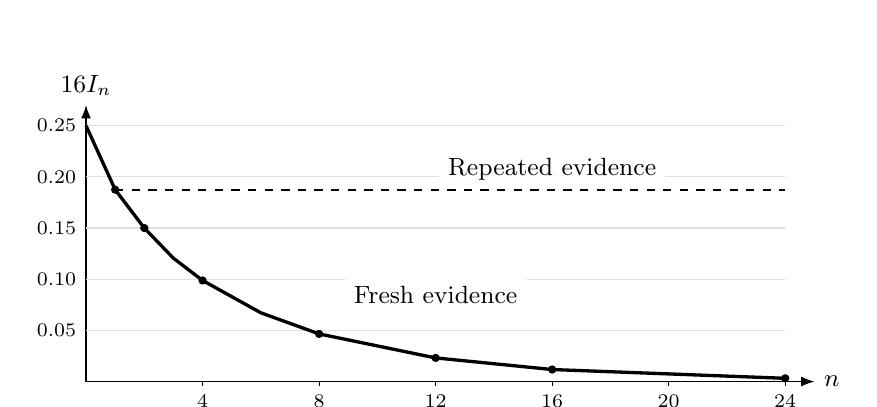
\begin{tikzpicture}[x=.37cm,y=13cm,>=Latex]
\draw[->] (0,0)--(25,0) node[right,font=\small]{$n$};\draw[->] (0,0)--(0,.27) node[above,font=\small]{$16I_n$};
\foreach \y in {0.05,0.10,0.15,0.20,0.25} {\draw[gray!25] (0,\y)--(24,\y);\node[left,font=\scriptsize] at (0,\y){\y};}
\foreach \x in {4,8,12,16,20,24}{\draw (\x,0)--(\x,-.004) node[below,font=\scriptsize]{\x};}
\draw[thick,dashed] (1,.1875)--(24,.1875);\node[above,font=\small,fill=white] at (16,.1875){Repeated evidence};
\draw[very thick] plot coordinates {(0,.25)(1,.1875)(2,.15)(3,.120536)(4,.098780)(6,.067207)(8,.046573)(12,.023113)(16,.011785)(24,.003208)};
\foreach \x/\y in {1/.1875,2/.15,4/.09878,8/.046573,12/.023113,16/.011785,24/.003208}{\fill (\x,\y) circle[radius=1.5pt];}
\node[font=\small,fill=white] at (12,.085){Fresh evidence};
\end{tikzpicture}
\end{center}
\textit{Figure 2.} Synthetic exact-risk calculation. An indefinitely deep redundant hierarchy stagnates. Conditional independence is an explicit model assumption, not an observed property of separately prompted AI roles.
\end{samepage}
\section{The computability frontier}\label{sec:computability}
The Universal Proof Horizons and Universal Settlement Horizons papers \cite{uph,ush} separate finite observable improvements from effective knowledge of their last occurrence. Here is a self-contained Professor analogue. This section concerns a changing sequence of repair graphs, not a conditional-expectation martingale for one fixed $Z$.
\begin{theorem}[The last-grade improvement obstruction]\label{thm:halting}
There is a uniformly computable family of finite-stage exact Professor grades $z_n(e)$, with at most one strict improvement and a pointwise limit for each index $e$, such that no uniform total algorithm computes their limiting grades to absolute error less than $1/16$.
\end{theorem}
\begin{proof}
Let $e$ encode a machine and input. At stage $n$, simulate that computation for $n$ steps. Use a finite directed graph with initial state $s$, intermediate state $u$, and terminal $t$, with unit edges $s\to u\to t$. Add the optional unit edge $s\to t$ exactly when the computation is observed to halt. Its admission can be backed by the finite halting trace, and all old edges persist. The graph is an abstract repair graph, not an assertion that this shortcut is available in an arbitrary formal calculus. Its horizon is $H_n(e)=2$ before discovery and $1$ thereafter. Set $\alpha=0$ and $h=1/\log2$. The exact grade is $z_n(e)=2^{-H_n(e)}\in\{1/4,1/2\}$ and is uniformly computable. The limit is $1/2$ if the computation halts and $1/4$ otherwise. Any proposed uniform approximation within $1/16$ separates the two values by threshold $3/8$ and decides the halting problem. Contradiction.
\end{proof}
\begin{corollary}
There is no uniform total procedure that returns a stage after the final strict grade improvement in this family.
\end{corollary}
\begin{proof}Given such a stage, compute the grade there and distinguish $1/4$ from $1/2$, again deciding halting.\end{proof}
This is a precise case in which access to the \emph{limit} would supply classical oracle power. It does not follow that every limiting probabilistic Professor has such power, or that a physical infinity of sequential evaluations executes in finite time. Each finite stage remains ordinary computation. Convergence is pointwise in the index, not uniform: for any finite stage there exists an index that halts only later, leaving an error of $1/4$. In particular there is no computable per-instance stabilization bound or modulus achieving error strictly below $1/4$ throughout this family. For this specific family, a halting oracle computes the limiting grade exactly, and an oracle returning the limiting grade with the stated accuracy computes the halting decision.
\subsection{A stationary posterior variant}
The same separation can be illustrated within the probabilistic setting without asserting that changing grades form a martingale. Fix a binary hidden world $X$ with equal prior probabilities and let $Z=1/4+X/4$. For each fixed machine index $e$, the authorized observation rule at level $n$ reveals nothing about $X$ until the computation has halted within $n$ steps; thereafter it reveals $X$ exactly. For that fixed $e$, the conditional means equal $3/8$ before revelation and $Z$ afterwards. Along the specified world $X=1$, each finite value is uniformly computable in $e,n$, but its limit is $1/2$ on halting indices and $3/8$ otherwise. Uniformly approximating these limits with error less than $1/32$ would decide halting. The hierarchy is a bounded martingale for each fixed experiment; the nonhalting experiments retain positive residual ignorance ($1/64$). The input to the oracle question is the machine index together with the specified world, not a claimed effective description of an unknown probability law. Even the infinite observation transcript on that world is uniformly computable as a sequence (each entry uses bounded simulation); knowing its entire limiting information is not the same as having an algorithm to decide whether a revelation will ever occur. Noncomputability of a limit and zero residual ignorance are logically distinct.
\section{When is another Professor worth its cost?}
The original manuscript's Sections 17, 22, and 25 charge awareness and resource allocation. Thus an infinite theoretical hierarchy is not a prescription to run infinitely many evaluators. In a static one-step review, suppose a proposed next level has known positive cost $c_n$ in a fixed unit. Let $\lambda>0$ convert that cost to squared-error units. The expected benefit of the next review, conditional on the existing evidence, is
\[
 D_n=V_n-\E[V_{n+1}\mid\F_n]
     =\E[(P_{n+1}-P_n)^2\mid\F_n].
\]
The equality follows by expanding $Z-P_n$ and applying conditional orthogonality as in Theorem~\ref{thm:convergence}. An exact one-step value test for strict preference to review over stopping is $D_n>\lambda c_n$ (equality gives indifference), under an additive objective of expected squared grade error plus review cost. This is not a general stopping theorem: two reviews may be useful jointly even if the first alone gives little information. A full sequential policy must compare continuation options and account for all costs and their effect on the ATP's search budget.

If each additional review costs at least $c>0$, any policy with finite expected total review cost has finite expected review count, hence terminates almost surely. In the synthetic two-world example, consider a stopping policy using only the observed signals and, if randomized, independent auxiliary randomness. At each finite stopping stage both worlds assign positive probability to every finite signal string. Their laws on stopped finite transcripts (including the independent randomness) are mutually absolutely continuous, by decomposing any event by the stopping stage and signal string. Thus a report based on the stopped transcript cannot equal two distinct true grades almost surely in their respective worlds. An almost-surely finite policy cannot reproduce the limiting exact oracle with probability one under the two-world prior. A fixed budget may rationally select level 1 or level 2 even if level infinity is mathematically meaningful.
\section{Oraclehood: what has and has not been established}
The proposed hierarchy separates three notions rather than defining all of them as classical oracles.
\begin{center}
\begin{tabularx}{\linewidth}{@{}>{\raggedright\arraybackslash}p{.24\linewidth}>{\raggedright\arraybackslash}X@{}}
\toprule
Notion & Operational or mathematical criterion\\\midrule
Information-relative limiting Professor & $P_\infty$ minimizes expected squared grade error among estimators using $\F_\infty$. The limit exists under the stated contract; residual ignorance may be positive.\\
Exact grading oracle & $Z$ is determined by $\F_\infty$ almost surely. Exact recovery concerns one declared grading problem, not all mathematical truth.\\
Noncomputable oracle access & An oracle interface answers a specified function by assumption. Theorem~\ref{thm:halting} supplies a function equivalent to the halting set under effective reductions, so that access strictly exceeds ordinary computability.\\
\bottomrule
\end{tabularx}
\end{center}
In classical computability theory an oracle may also answer a computable set; the third row specifically concerns noncomputable oracle power. The second property does not imply the third: a finite graph with a known complete edge list has computable shortest paths. The third supplies no claim of self-awareness, nor does it imply omniscience outside the declared problem. We retain the user's broader idea of ignorance-minimizing oraclehood as a research definition; the squared-error criterion here is one concrete candidate, not its universal replacement.
\begin{conjecture}[Useful recursive Professor architecture]
On some declared families of held-out ATP problems, an authorized level-2 or higher Professor that gathers complementary evidence about capital, repair geometry and calibration can improve verified settlement per fully charged resource budget relative to a matched level-1 architecture.
\end{conjecture}
This is an empirical conjecture. A lower grade risk alone does not imply increased theorem-proving performance. A Professor that predicts a useless score perfectly may still be useless. Establishing the connection requires a separately specified decision policy and benchmark.
\section{A first experiment and open problems}
Freeze a verifier, theory, target family, capital map, repair costs, score weights, search policy, and complete resource accounting. Begin with a proof-side benchmark, as the parent article recommends. On finite solved graphs, independently calculate exact horizons and ground-truth grades; on real held-out proofs, distinguish graph-local labels from unknown global horizons. Avoid leaking retrospective labels into live evaluations.

Compare four arms with equal total budget: (A) ordinary deterministic Professor baseline; (B) probabilistic level 1; (C) level 2 with only the same available evidence; (D) level 2 with an authorized complementary observation or independent checked bound. A fifth arm may compare levels 3--4 if resources allow. Count the cost of all reviews, prompts, verification, and information acquisition. Record squared-error grade loss where ground truth is known, uncertainty calibration, verified settlement rate and cost, certified interval coverage, and the frequency and value of grade revisions. Preserve failed trials and an independent search fallback. A common model must be tested, not inferred from agreement among related AI agents. Neither the existing DATA MIND configuration nor a deployed Picard implementation is modified by this proposal.

\textbf{Open questions.} Can evidence acquisition be arranged to make the limiting grade identifiable without allowing an unauthorized source? Can a finite Professor certify that a higher review is unnecessary on a nontrivial family? What is the weakest effective evidence contract yielding a useful convergence rate? Can the recursive evaluation target include the quality of the grading map $Q$ without changing the original contract in mid-episode? How do correlated errors and shared model training affect effective depth? Which classes of limit grades lie at which computability degrees?

\textbf{Claim status.} The martingale and orthogonality results are standard probability theory applied to the proposed contract. The graph obstruction is an explicit halting reduction. The numerical example is an exact finite synthetic calculation. The empirical architecture, general ignorance concept and utility conjecture remain open; no classical oracle or autonomous self-upgrading ATP has been implemented or demonstrated here.

\clearpage
\section*{Research provenance and AI disclosure}
This audited sequel develops Brian Tenneson's recursive-Professor proposal from his September 3 manuscript. Picard--CIIP is the name of a ChatGPT conversational research protocol, not a separately deployed theorem prover. The draft includes paper-level arguments and a reproducible synthetic numerical example, and has received a repeated AI-assisted Atlas-style proof and consistency review. It has not undergone independent peer review or formal machine proof checking. No claim of priority over established probability, scoring, or computability results is made. All deployment decisions remain external to the mathematical framework.
\section*{Atlas v2 audit record}
The source and rendered manuscript were reviewed in two passes: first the grading contract, conditional-expectation identities, example and halting construction; then the repaired statements, proofs, numerical outputs and scope. The core convergence theorem and its exactness criterion were retained. This edition makes the following substantive corrections and clarifications:
\begin{itemize}
\item Replaces ambiguous uniform-limit language with pointwise convergence and noncomputability of the indexed limit, and distinguishes noncomputable oracle access from ordinary oracle terminology.
\item Specifies fixed weights, common-law semantics, version choices, and the difference between the aggregate information and a practical Professor's report. Adds exact excess-risk accounting and sufficient conditions for convergence of approximate graders.
\item Separates scalar-grade recovery from horizon recovery and certification; supplies a direct proof of shrinking-envelope recovery and a conditional variance bound.
\item Makes the stopping claim precise for signal-adapted policies with independent randomness, clarifies the strict one-step decision criterion, and records the finite-model risk bound.
\item Recomputes the synthetic results using exact arithmetic, cross-checks them with a likelihood-recursion calculation, and verifies the printed numerical entries and graph coordinates to their stated precision.
\end{itemize}
No remaining mathematical defect was identified in this scoped review of the revised claims under their stated assumptions. This is not a proof of the manuscript's freedom from errors. No operational ATP benchmark, independent peer review, or machine-checked formalization was performed. The parent article, the original draft, and deployed systems remain unchanged.
\clearpage
\begin{thebibliography}{9}\small
\bibitem{partial} B. Tenneson, \emph{Partial Credit on Settlement Geometry: Proof Compass, Mathematical Capital, Directed Awareness, and Marginal Resource Allocation in DATA MIND}, 3 September 2026, supplied 24-page manuscript, especially Sections 2--12, 17, 22, 24--26. \href{https://btenneson.github.io/pub/cs.LO_Logic_in_Computer_Science/partial_credit_on_settlement_geometry_data_mind/}{Publication page}.
\bibitem{uph} B. Tenneson, \emph{Universal Proof Horizons for a Single ATP}, research draft 0.3, revised 30 October 2026, especially the last-breakthrough noncomputability theorem. \href{https://btenneson.github.io/pub/cs.LO_Logic_in_Computer_Science/universal_proof_horizons_single_atp_0_3/}{Publication page}.
\bibitem{ush} B. Tenneson, \emph{Universal Settlement Horizons}, corrected research synthesis 002. \href{https://btenneson.github.io/pub/cs.LO_Logic_in_Computer_Science/universal_settlement_horizons_002/}{Publication page}.
\bibitem{password} B. Tenneson, \emph{Password-Seeking with AMLD+0: Singleton Enumeration, SAT, and CNF Pruning}, 30 September 2026. \href{https://btenneson.github.io/pub/cs.LO_Logic_in_Computer_Science/password_seeking_with_amld_plus_0_singleton_enumeration_sat_cnf_pruning/}{Publication page}.
\bibitem{williams} D. Williams, \emph{Probability with Martingales}, Cambridge University Press, 1991, Chapters 9 and 14 (conditional expectation and L\'evy's upward theorem).
\bibitem{brier} G. W. Brier, ``Verification of forecasts expressed in terms of probability,'' \emph{Monthly Weather Review} 78(1), 1--3 (1950).
\bibitem{hoeffding} W. Hoeffding, ``Probability inequalities for sums of bounded random variables,'' \emph{Journal of the American Statistical Association} 58(301), 13--30 (1963).
\end{thebibliography}
\end{document}
